\documentclass[a4paper,12pt]{article}
\usepackage{graphicx}
\usepackage{hyperref}
\usepackage{geometry}
\geometry{margin=1in}

\title{Architectural Requirements Document}
\date{}

\begin{document}

% Cover Page
\begin{titlepage}
    \centering
    
\includegraphics[width=\textwidth]{coverPage.png}
    \vfill
    \maketitle
    \vfill
\end{titlepage}

\tableofcontents
\newpage

\section{Architectural Design Strategy}

\subsection{Background}
For our logistics optimization system, we aimed to develop a comprehensive solution that addresses the unique needs of managing and optimizing the placement of goods in logistics trucks. Our system leverages dynamic algorithms and machine learning models to enhance efficiency and space management. This application will assist logistics managers in predicting office capacities and managing desk allocations to prevent overbooking. Given the diverse and demanding requirements of such a system, we have focused on ensuring high performance, scalability, security, reliability, and usability.

\subsection{Architectural Decisions}
The architectural decisions have been based on the quality requirements of the system. We have used the quality requirements (listed in our System Requirements Specification: SRS) to identify our quality requirements which were used to identify our architectural patterns.

\section{Architectural Quality Requirements}
\subsubsection*{NF1. Performance:}
\begin{itemize}
    \item The application shall have fast response times for user interactions.
    \item The application's database operations, implemented with Supabase, should have efficient query execution times to ensure quick retrieval and storage of data.
    \item The system should return the optimal packing route within 2-5 minutes of the provided configuration/input parameters.
    \item The real-time 3D render should reflect optimizations in real time without any delay or buffering.
\end{itemize}

\subsubsection*{NF2. Scalability:}
\begin{itemize}
    \item The backend infrastructure, particularly the database layer hosted on Supabase, should be capable of handling increasing loads as the user base expands.
    \item The system should be scalable in the sense the algorithm could potentially be used for packing cargo trains, or shipping containers.
\end{itemize}

\subsubsection*{NF3. Security:}
\begin{itemize}
    \item All user authentication and authorization processes, including registration, login, and password reset, must follow the best practices for safe transfer and storage of sensitive user information.
    \item Data stored in the Supabase database must be encrypted to protect user privacy and comply with relevant data protection regulations.
\end{itemize}

\subsubsection*{NF4. Reliability:}
\begin{itemize}
    \item Error handling mechanisms shall be implemented to handle erroneous input and provide helpful feedback to users in case of unexpected errors.
    \item Continuous integration and deployment pipelines (CI/CD) shall be set up using GitHub Actions to ensure reliable software releases.
\end{itemize}

\subsubsection*{NF5. Usability:}
\begin{itemize}
    \item The application shall have an intuitive and user-friendly interface to ensure ease of use for all user types, including logistics managers, truck drivers, and warehouse staff.
    \item The interface should be accessible and provide a consistent user experience across various devices and screen sizes.
    \item The system shall provide clear instructions and feedback to users, guiding them through the process and informing them of any errors or required actions.
    \item The system shall provide real-time updates to users, ensuring they are always informed of the current status and any changes in the packing process.
\end{itemize}

\section{Architectural Strategies}
The Extended Planning Instrument for Unpredictable Spaces and Environment is coupled with the following architectural patterns; layered, API gateway, and service-oriented architecture of the software. The different architectural patterns are shown in the following diagram:

\begin{figure}[h]
    \centering
    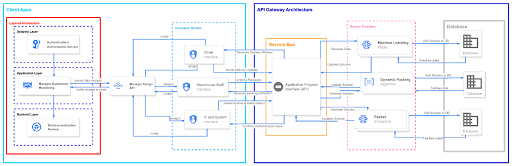
\includegraphics[width=\textwidth]{architecturalDiagram.png}
    \caption{Architectural Patterns}
\end{figure}

The system is a compilation of a three-tier layered architecture, which is formed by the security, application, and backend layers of the system. Each of the layers is responsible for a different task to which their layer entails. The Security Layer is responsible for the Authentication and Authorization of the system's security. The Layer then interacts with the layer below it, which is the Application Layer. This is the first-hand interface of the system. The manager dashboard has access to the presentation of the entirety of the system. This then interacts with the layer below it which is the backend of the system. This compiles the Delivery Instructions developed by the microservices at the backend of the system.

Another architecture pattern that is found is the Service-Oriented architecture, where the Service Consumers would be the Driver, Warehouse Staff, and IT and System Interfaces.

Furthermore, the Service Providers would be the Machine Learning Model, Dynamic Packing Algorithm, and Packer Instructions. The Service Bus in the service-oriented architecture would be the API, which serves as a gateway from the service provider and the relevant service consumer.

The last architecture pattern we found is the API Gateway Architecture. The different interfaces in the system are the actual Client Application and the Microservices are the different algorithms used to solve the problem. As a gatekeeper that ensures only authorized requests get through, an API is used to connect the Client Application and the Microservices of the system together.

The API serves as a centralized entry point into the Machine Learning Model, Dynamic Packing Algorithm, Packer Instruction. This acts as a mediator between the clients of the different interfaces and the microservices, providing a unified interface to access them. This kind of approach performs several key functions, including security enforcement, request routing, protocol translation, load balancing, and monitoring of the system.

\section{Architectural Patterns and Non-Functional Requirements}
Mitigating the architectural pattern with our non-functional requirements of the system is crucial. This ensures that the system is not only functionally correct, however, it also meets the desired quality attributes. Here is how our three architectural patterns, Layered, API Gateway, and Service-Oriented Architecture affect our systems Non-Functional Requirements:

\subsection{Performance}
Having a three-tier layered architecture enables us to optimize each of the three layers to its specific performance. For example, the Security Layer of the architecture uses efficient authentication and authorization. By separating concerns of the system, a layered architecture reduces the overall complexity of each component. The simplification of each component leads to more efficient code and better performances when it comes to developing the system from scratch. When developing the software, we focused on optimizing specific aspects of the system.

The separation of concerns allows each layer to focus on specific tasks, which can lead to more efficient code and optimized performance. For example, the Security Layer can implement efficient authentication and authorization mechanisms without affecting the performance of the Application and Backend layers.

The API Gateway pattern of the system manages request routing, load balancing, and caching to improve the overall performance of the system. By this, efficient performance between the Client Application and the Microservices is improved by the efficient management of the system's requests. Henceforth, the performance of the API is critical to ensure that it responds quickly and efficiently to user requests.

Managing the API in a system that has different sets of interfaces and endpoints can be time-consuming. Using API Gateway we saved heaps of time and effort by centralizing the API controls by merging all the different interfaces under one umbrella solution offering greater flexibility and efficiency for various use cases.

Routing requests through a single entry point has worked wonders in simplifying our system, especially when dealing with multiple backend services. By unifying the different interfaces of the system and grouping multiple microservices in the backend, it takes a lot of load off developing and using the application.

SOA allows for the decomposition of complex systems into smaller, manageable services. This enables independent optimization of each service, potentially improving the overall system performance.

\subsection{Scalability}
Changes in one layer (e.g., updating the security protocols) do not directly affect other layers, providing a stable environment where updates and maintenance can be handled more effectively.

The API Gateway serves as a vital tool for efficiently managing an API by distributing the workload effectively. By spreading incoming requests across multiple instances of our system API, it prevents overloading and boosts scalability and availability. This, in turn, enhances user experience by ensuring consistent and reliable service delivery.

Additionally, an API Gateway acts as a central point for authentication, monitoring, and traffic management, streamlining the process of handling API requests and responses. Its role in simplifying complex architectures and facilitating communication between different microservices makes it a key component in building robust and high-performing applications that can be easily scaled up or down depending on adding or removing microservices in the actual system.

The independence of services means that changes or failures in one service do not necessarily affect others, contributing to the system's stability.

\subsection{Security}
A dedicated Security Layer enhances security by centralizing all security-related functions, ensuring consistent enforcement of security policies across the system.

The API Gateway acts as an effective gatekeeper within our system. Using an API, we have a single point of entry to which we effectively enforce security policies such as ensuring only authorized requests reach the backend services. Building the system, we understand that a possible weak point for any application is the handling of data. Henceforth, the API Gateway acts as an efficient tool to safeguard against cyber threats by processing any incoming traffic through low latency traffic routing before it reaches its ultimate destination.

SOA can include multiple layers of security across different services, providing granular control over access and ensuring secure data transactions.

\subsection{Reliability}
By isolating functionalities into different layers, the system becomes more reliable as failures in one layer do not necessarily propagate to others.

By centralizing error handling and providing fallback mechanisms, the API Gateway can improve the reliability of the system. It can also retry requests or provide alternative responses in case of failures.

The decoupled nature of services in SOA enhances reliability, as services can be independently scaled, replaced, or upgraded without disrupting the entire system.

\subsection{Usability}
The layered approach can improve usability by allowing for a more focused and clear design of the user interfaces in the Application Layer, while other layers handle more complex processing.

It provides a unified and consistent interface for clients, making it easier for developers to interact with the system. This can lead to better user experiences and easier integration with other systems.

It allows for flexible integration of new services and can provide tailored interfaces for different types of users or clients, improving usability.

\section{Design Patterns Used}
\subsection{Facade}
The Manager Dashboard Interface will act as the facade, providing a simplified and unified interface for the logistics manager to interact with the underlying subsystems like the Dynamic Packing Algorithm Service, Machine Learning Model Service, Packer Instructions Service, and Delivery Instructions Service.

The facade will expose methods for the manager to input constraints, preferences, and priorities for the packing algorithm. It will communicate with the Dynamic Packing Algorithm Service, translating the user input and retrieving the generated packing solution for presentation.

The facade will also provide an interface for the manager to review and provide feedback on the packing solutions. It will collect this feedback and pass it to the Machine Learning Model Service to improve the algorithm over time. Additionally, it will retrieve and display insights or recommendations from the Machine Learning Model Service.

Furthermore, the facade will allow the manager to access packing instructions for warehouse staff and delivery instructions for truck drivers by communicating with the respective services and presenting the information in a user-friendly format.

By acting as the facade, the Manager Dashboard Interface will handle the complexities of communicating with the subsystems, promoting better code organization, readability, and separation of concerns. It also facilitates easier maintenance and extensibility, as changes to the subsystems won't affect the facade's interface as long as the contracts remain unchanged.

\subsection{Singleton}
The Singleton Pattern ensures that a class has only one instance and provides a global point of access to that instance. This is particularly useful for managing shared resources and maintaining a consistent state across the system.

A singleton database connection can efficiently manage database connections, optimizing resource utilization and maintaining connection limits for improved performance and stability.

Security services managing authentication and authorization also benefit from the Singleton Pattern by providing a consistent and universally accessible point of control, enhancing overall security.

\section{Architectural Constraints}
\subsection{Data Constraints}
The system must utilize specific datasets provided in the linked documents for developing and training the machine learning models. These datasets form the foundation for the algorithm's learning and optimization processes. All data must be handled in compliance with relevant data protection regulations. Sensitive information must be encrypted, and access must be restricted to authorized personnel only.

\section{Technology Choices}
\subsection{Backend}
\begin{itemize}
    \item Languages \& Frameworks: Python
    \item Database: PostgreSQL on Supabase
    \item Machine Learning: TensorFlow
    \item APIs: RESTful APIs
\end{itemize}

\subsection{Frontend}
\begin{itemize}
    \item Languages \& Frameworks: JavaScript, Vue, PrimeVue, Tailwind CSS
    \item Visualization: Three.js
\end{itemize}

\subsection{DevOps}
\begin{itemize}
    \item Version Control: Git, GitHub
    \item CI/CD: GitHub Actions
    \item Containerization: Docker
    \item Cloud Platforms: Vercel
\end{itemize}

\subsection{Security}
\begin{itemize}
    \item Auth/Access Control: OAuth 2.0, JWT
    \item Encryption: SSL/TLS
\end{itemize}

\subsection{Collaboration}
\begin{itemize}
    \item Communication: Discord, WhatsApp, Google Drive
    \item Project Management: GitHub Project Board
    \item Documentation: Google Docs
\end{itemize}

\end{document}
